\documentclass[11pt,a4paper]{article}

\usepackage[utf8]{inputenc}
\usepackage[T1]{fontenc}
\usepackage[french]{babel}
\usepackage[a4paper,margin=2.3cm]{geometry}
\usepackage{graphicx}
\usepackage{amsmath,amssymb}
\usepackage{booktabs}
\usepackage{float}
\usepackage{subcaption}
\usepackage{caption}
\usepackage{xcolor}
\usepackage[hidelinks]{hyperref}

\graphicspath{{figures/}}
\captionsetup{font=small,labelfont=bf}

\title{\vspace{-1.5cm}\textbf{Classification d'images de chiens :\\ d'un pipeline classique aux réseaux profonds}}
\author{Romain Ben \and Zouhair Saitout \and Evrard Lecureur}
\date{Polytech Nice Sophia --- MAM3 --- Introduction au Machine Learning\\
Encadrants : Mahmoud Elsawy \& Jean-Luc Bouchot (INRIA)\\
Juin 2026}

\begin{document}

\maketitle

\begin{abstract}
\noindent Dans ce projet de Machine Learning, on cherche à classifier des images de chiens parmi six races issues du jeu de données Stanford Dogs Dataset. Notre travail s'est structuré autour de deux approches : un pipeline classique et du transfer learning. Pour le pipeline classique, après un prétraitement des images (rognage et redimensionnement avec conservation des proportions), on a extrait des descripteurs en combinant une PCA et des histogrammes de gradients orientés (HOG). On a ensuite comparé deux algorithmes : les k-plus proches voisins (kNN) et les SVM (Support Vector Machines), en étudiant l'impact de la normalisation et en optimisant les hyperparamètres. Nos meilleurs modèles classiques plafonnent autour de $59\%$ de précision sur l'ensemble de test, limités par la forte ressemblance entre certaines races. Enfin, on a utilisé le transfer learning à l'aide d'un réseau pré-entraîné VGG16, ce qui nous a permis d'atteindre un score de $98\%$ de bonnes réponses.
\end{abstract}

\section{Introduction et premier regard sur les données}

L'objectif de ce projet est de concevoir un système de classification automatique de races de chiens à partir d'images. On travaille sur un jeu de données extrait de Stanford Dogs Dataset, contenant six races : \textit{Chihuahua}, \textit{basset}, \textit{Kerry blue terrier}, \textit{groenendael}, \textit{malinois} et \textit{chow}. En plus des images, on a à disposition des fichiers XML contenant les coordonnées des boîtes englobantes (\textit{bounding boxes}) délimitant la position du chien sur chaque photo.

\paragraph{Les classes sont-elles équilibrées ?} Avant de lancer nos entraînements, on a vérifié si notre jeu de données était équilibré, car un fort déséquilibre pourrait fausser nos métriques d'évaluation. On a calculé l'entropie de Shannon de la distribution des classes :
\begin{equation}
H(P) = -\sum_{i} p_i \ln(p_i),
\end{equation}
où $p_i$ est la proportion d'images de la race $i$. Pour six classes, la valeur maximale théorique (cas où toutes les races sont parfaitement équiréparties) est $\ln(6) \approx 1{,}792$. On obtient expérimentalement $H = 1{,}7863$, ce qui est extrêmement proche du maximum. La Figure~\ref{fig:balance} montre le nombre d'images par race. Comme les effectifs varient seulement entre $150$ et $196$ images, on peut considérer que le dataset est bien équilibré. On pourra donc utiliser la précision (accuracy) globale pour comparer nos modèles sans risquer de biais lié à une classe ultra-majoritaire.

\begin{figure}[H]
\centering
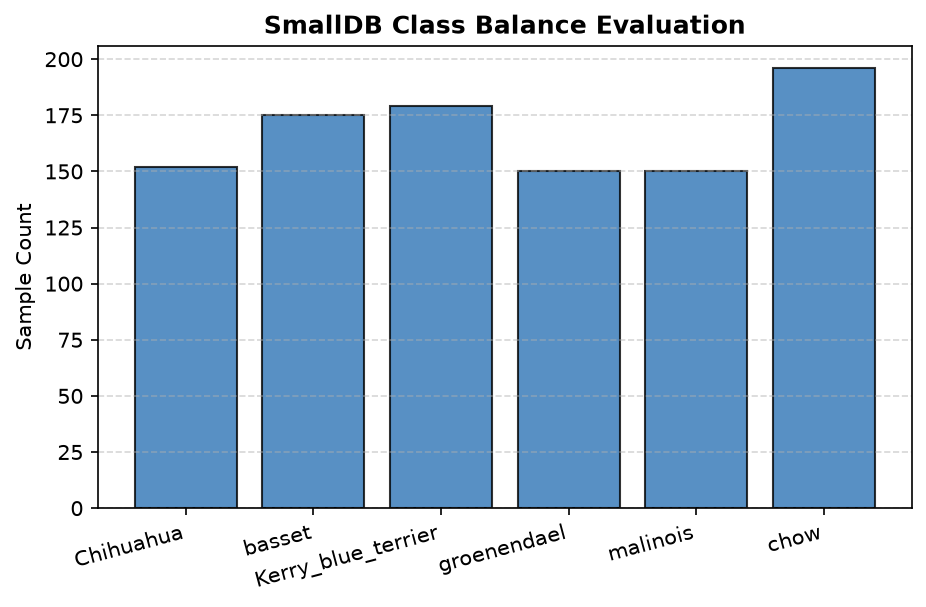
\includegraphics[width=0.62\textwidth]{class_balance.png}
\caption{Nombre d'images par race dans \textit{SmallDB}. Les six races ont des effectifs proches, ce qui confirme l'entropie quasi maximale.}
\label{fig:balance}
\end{figure}

\section{Préparation des images}

\subsection{Découpage autour du chien}

Les images d'origine contiennent souvent beaucoup d'informations inutiles pour la classification (de l'herbe, des meubles, d'autres objets). Pour éviter que ces éléments perturbent l'apprentissage des modèles, on utilise les coordonnées fournies dans le fichier XML associé à chaque image afin de la rogner (\textit{crop}) autour du chien (Figure~\ref{fig:bbox}). Cela permet de recentrer les descripteurs uniquement sur l'animal.

\begin{figure}[H]
\centering
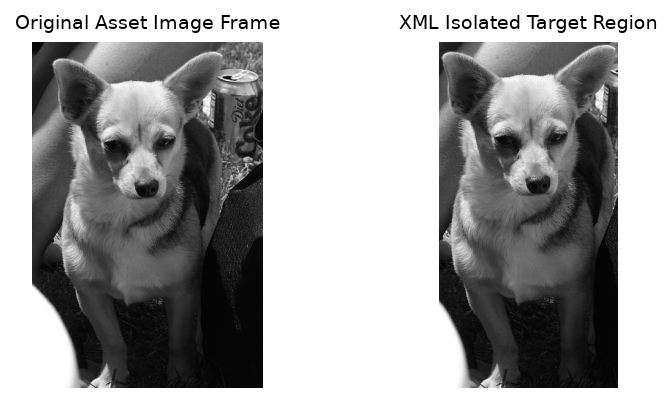
\includegraphics[width=0.7\textwidth]{bounding_box_crop.png}
\caption{Découpage d'une image autour de la zone du chien. À gauche la photo d'origine, à droite la partie gardée grâce au cadre indiqué dans le fichier XML.}
\label{fig:bbox}
\end{figure}

\subsection{Mise à la même taille sans déformer}

Nos classifieurs ont besoin d'images de taille identique : on les ramène donc à une taille fixe de $64 \times 64$ pixels dans notre code final. Si on redimensionne directement sans précaution, le chien se retrouve écrasé ou étiré. Pour éviter cela, on garde les proportions de l'image en la mettant à l'échelle avec le facteur $\min(h_r, w_r)$ où $h_r = H_{\text{cible}}/h$ et $w_r = W_{\text{cible}}/w$, puis on la place au centre d'un fond de taille fixe. Il reste alors des bandes vides à remplir, et on a testé plusieurs méthodes : le noir, le blanc, le prolongement des pixels du bord (\textit{continuous}), l'effet miroir (\textit{mirroring}), et la propagation de flou (\textit{propagated blur}). La Figure~\ref{fig:padding} illustre ces choix sur trois images de formes différentes.

\begin{figure}[H]
\centering
\includegraphics[width=0.7\textwidth]{preprocessing_comparaisonV2.png}
\caption{Comparaison des façons de remplir les bords après redimensionnement. Le remplissage continu prolonge la couleur du bord, ce qui évite de créer de fausses bordures qui gêneraient le calcul des contours.}
\label{fig:padding}
\end{figure}

Pour la suite, on a choisi d'utiliser le remplissage par propagation de flou (\textit{propagated blur}) combiné au mode miroir ou bord. En effet, un remplissage noir ou blanc uniforme crée une frontière très nette avec le bord de l'image d'origine. Cette transition brusque génère des gradients artificiels qui viendraient fausser les descripteurs HOG en faisant croire à la présence de contours importants sur les contours du cadre.

\section{Calcul des caractéristiques}

\subsection{La PCA}

Une image en niveaux de gris de $64 \times 64$ pixels représente un vecteur de $4\,096$ variables, ce qui est trop grand pour des algorithmes simples comme le kNN. On utilise donc l'analyse en composantes principales (PCA) pour réduire la dimensionnalité tout en conservant le maximum d'information (variance). La Figure~\ref{fig:scree} montre la variance portée par chaque axe (diagramme des éboulis de la PCA globale). On remarque que les premières composantes concentrent une grande partie de la variance cumulée, ce qui montre qu'il y a beaucoup de redondance dans les pixels des images d'origine.

\begin{figure}[H]
\centering
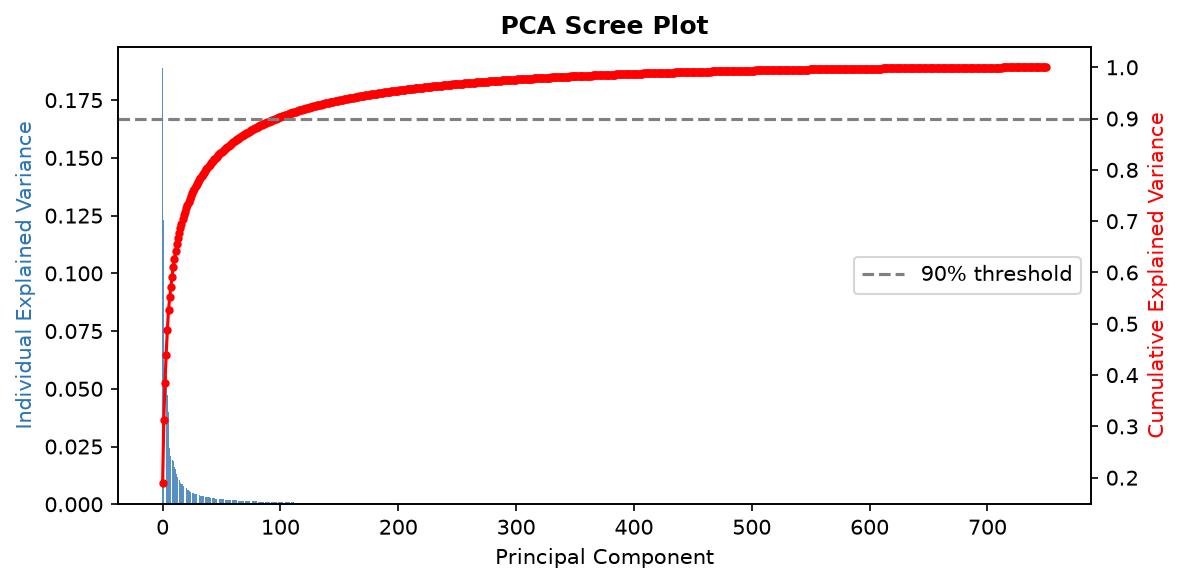
\includegraphics[width=0.78\textwidth]{pca_reconstruction.png}
\caption{Part d'information portée par chaque axe de la PCA. En bleu, l'information de chaque axe pris seul ; en rouge, le total cumulé. La ligne en pointillés marque le seuil de $90\%$.}
\label{fig:scree}
\end{figure}

\paragraph{Reconstruire une image.} La Figure~\ref{fig:approx} montre ce qu'on obtient quand on reconstruit une image à partir de ses $k$ premiers axes :
\begin{equation}
\hat{x}_k = \bar{x} + \sum_{i=1}^{k} \langle x - \bar{x},\, u_i \rangle\, u_i,
\end{equation}
avec à chaque fois l'écart $L_2 = \lVert x - \hat{x}_k \rVert$ entre l'image d'origine et sa reconstruction. La Figure~\ref{fig:approx} montre cette reconstruction pour différentes valeurs de $k$. On constate qu'avec très peu d'axes (ex: $k=10$), l'image reconstruite est très floue et ne conserve que la silhouette globale et la luminosité moyenne. Plus $k$ augmente, plus les détails fins réapparaissent et plus l'erreur L2 diminue.

\begin{figure}[H]
\centering
\includegraphics[width=0.92\textwidth]{pca_approximatrion.png}
\caption{Reconstruction d'une image avec de plus en plus d'axes $k$. L'image d'origine (en haut à gauche) réapparaît petit à petit, et l'écart $L_2$ diminue.}
\label{fig:approx}
\end{figure}

\paragraph{Est-ce que les races se distinguent ?} Si on projette l'ensemble des données sur les deux premiers axes principaux (Figure~\ref{fig:scatter}), on observe que les différentes races de chiens sont complètement mélangées. Il n'y a pas de groupes distincts par classe. Cela nous montre dès le départ que le problème de classification sera difficile à résoudre linéairement avec des descripteurs basiques.

\begin{figure}[H]
\centering
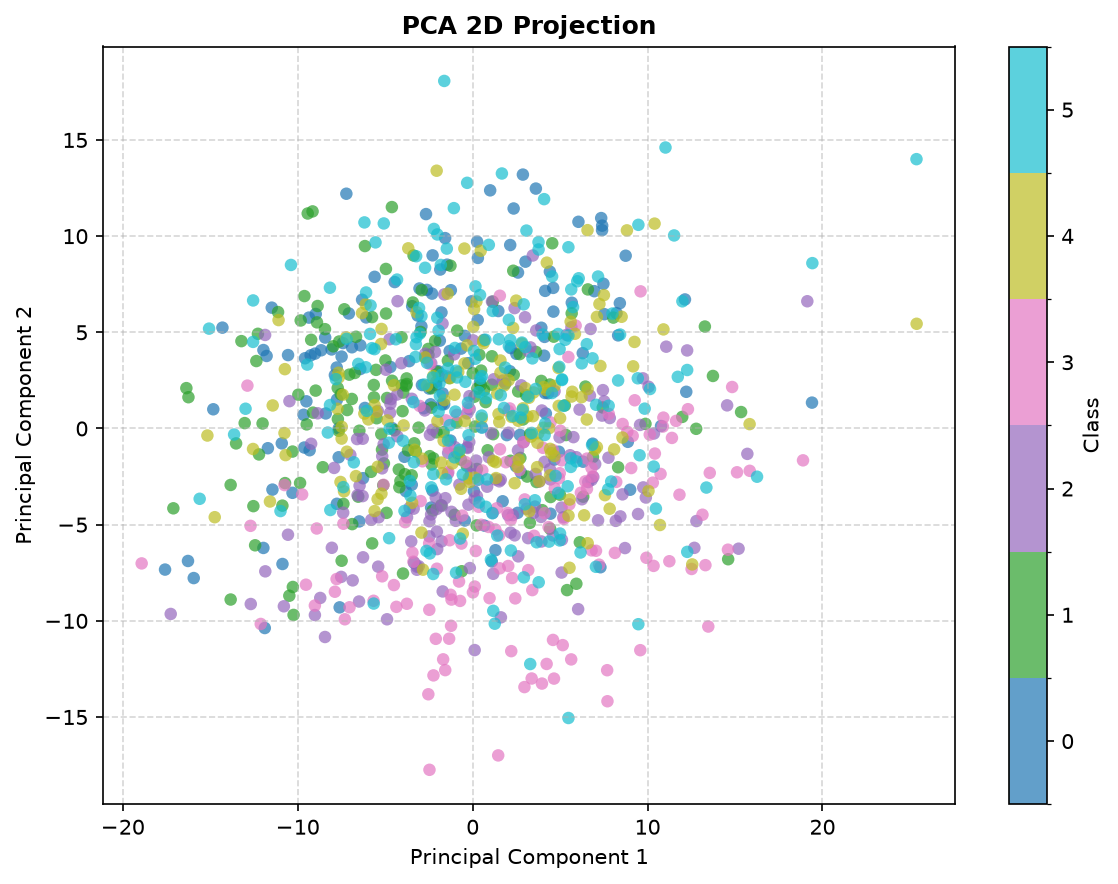
\includegraphics[width=0.62\textwidth]{pca_scatter_plots.png}
\caption{Toutes les images placées sur les deux premiers axes de la PCA, une couleur par race. Le mélange des couleurs montre que les races sont difficiles à séparer.}
\label{fig:scatter}
\end{figure}

\subsection{Le HOG}

Le descripteur HOG (Histogram of Oriented Gradients) permet de capturer les contours et les textures locales, ce que la PCA globale (qui s'intéresse surtout à l'intensité globale des pixels) a du mal à faire. On découpe l'image en petites cellules (une grille de $4 \times 4$ cellules dans notre cas), on calcule les gradients horizontaux $g_x$ et verticaux $g_y$ via des filtres de Sobel pour chaque pixel (Figure~\ref{fig:hog}), puis on construit un histogramme des orientations des gradients pondéré par leur intensité dans chaque cellule.

\begin{figure}[H]
\centering
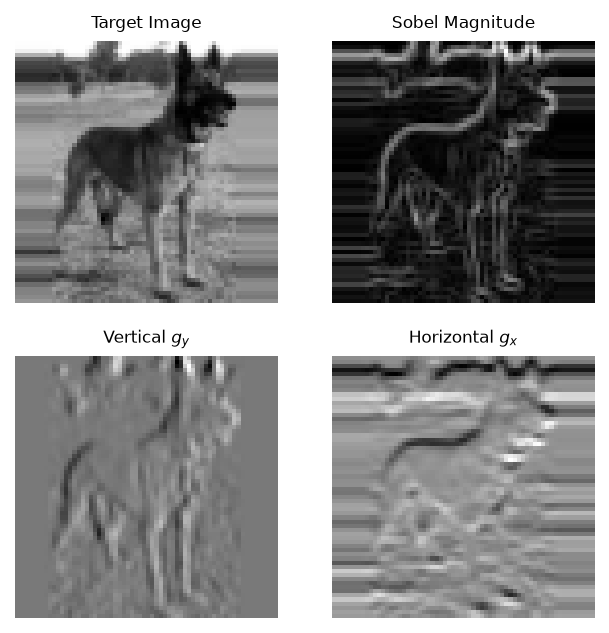
\includegraphics[width=0.6\textwidth]{sobel_hog.png}
\caption{Contours de Sobel utilisés par le HOG : la force du contour et ses deux directions $g_x$ et $g_y$. On distingue bien la silhouette du chien.}
\label{fig:hog}
\end{figure}

Pour représenter chaque image, on concatène les caractéristiques issues de la PCA (calculée par classe pour projeter sur les sous-espaces) et les descripteurs HOG. On obtient ainsi un vecteur combinant l'allure générale et les contours locaux.

\section{Classification avec le kNN}

\subsection{Pourquoi normaliser les données}

Les composantes issues de la PCA et les valeurs du HOG possèdent des ordres de grandeur très différents. Comme l'algorithme kNN repose sur le calcul d'une distance euclidienne dans l'espace des descripteurs, les variables ayant les plus grandes amplitudes numériques domineraient artificiellement la distance. Pour équilibrer la contribution de chaque descripteur, on applique un centrage-réduction (\texttt{StandardScaler}). La partie gauche de la Figure~\ref{fig:task6} montre que la normalisation améliore nettement les performances en faisant baisser la perte de Hamming sur le test.

\subsection{Modèle trop simple ou trop complexe ?}

La courbe centrale de la Figure~\ref{fig:task6} présente l'évolution des erreurs d'entraînement et de test en fonction du nombre de voisins $k$. On retrouve ici l'illustration classique du compromis biais-variance :
\begin{itemize}
\item Pour $k=1$, l'erreur d'entraînement est nulle car chaque image est son propre voisin le plus proche. Le modèle est en surapprentissage total.
\item Quand $k$ augmente, la frontière de décision se lisse, ce qui fait augmenter l'erreur d'entraînement. Sur le test, l'erreur commence par baisser avant de remonter légèrement pour les grandes valeurs de $k$, car le modèle devient trop simple (sous-apprentissage) et n'arrive plus à capturer la spécificité des classes.
\end{itemize}

\begin{figure}[H]
\centering
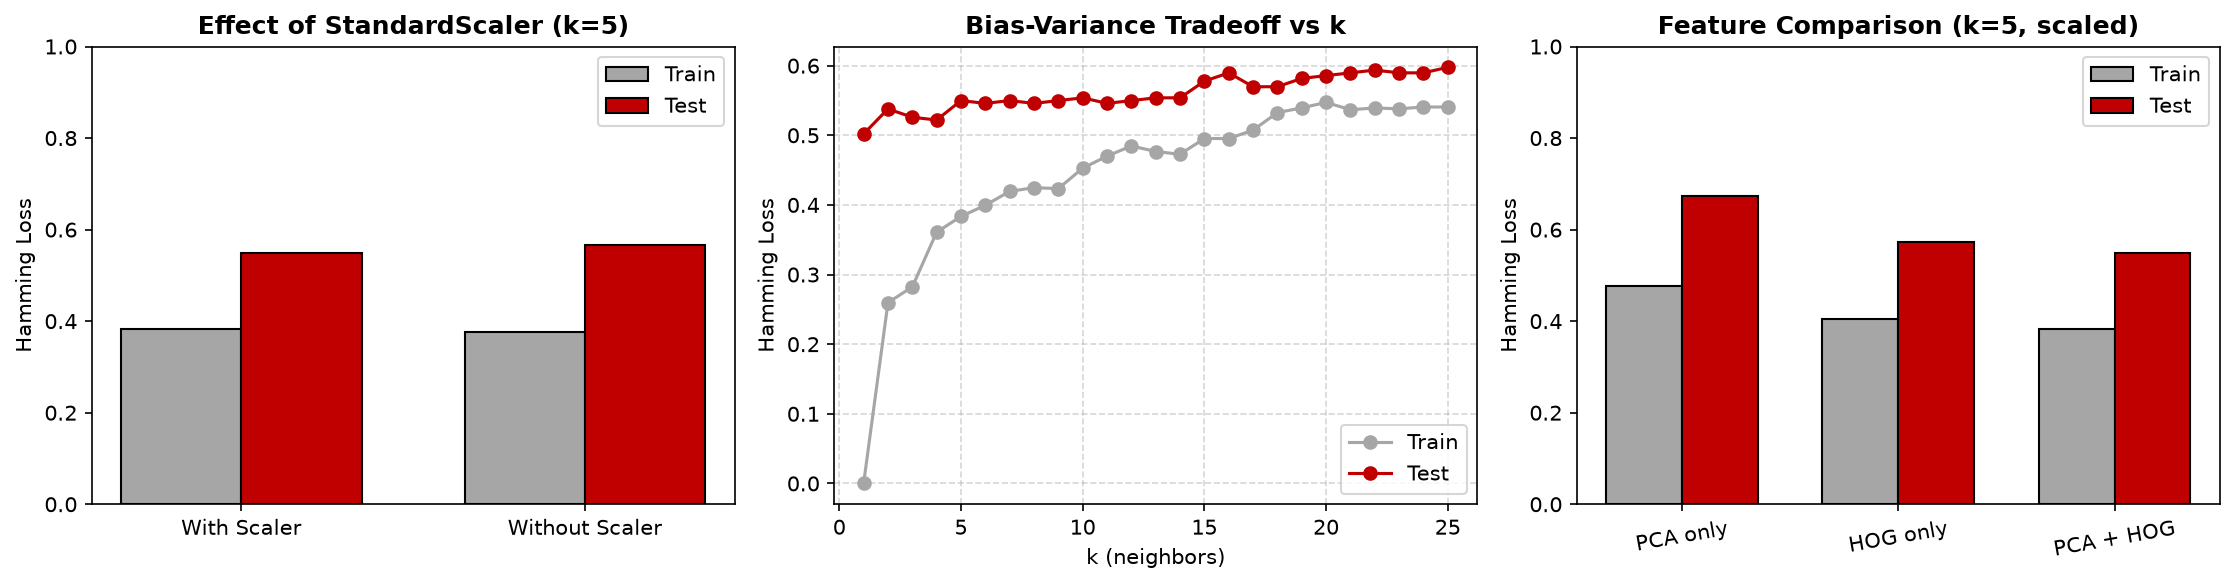
\includegraphics[width=\textwidth]{task6_analysis.png}
\caption{Étude du kNN. \textbf{Gauche} : effet de la normalisation. \textbf{Centre} : erreurs sur entraînement et test selon $k$. \textbf{Droite} : comparaison des caractéristiques (PCA seule, HOG seul, les deux ensemble).}
\label{fig:task6}
\end{figure}

\paragraph{Attention à la pondération par distance.} Si on utilise l'option \texttt{weights='distance'}, l'erreur d'entraînement reste nulle pour n'importe quelle valeur de $k$. C'est un comportement mécanique : lors de la prédiction sur un point de l'ensemble d'entraînement, ce point se trouve à une distance nulle de lui-même, ce qui lui donne un poids infini. Cela montre bien qu'il ne faut pas se fier à une erreur d'entraînement nulle pour évaluer un modèle.

\subsection{Apport des caractéristiques}

La partie droite de la Figure~\ref{fig:task6} présente une étude d'ablation des descripteurs (PCA seule, HOG seul, et PCA + HOG). La combinaison des deux caractéristiques donne la plus faible perte de Hamming sur l'ensemble de test. Cela montre que la forme globale (PCA) et les contours locaux (HOG) sont bien complémentaires.

\subsection{Où le modèle se trompe}

La matrice de confusion du kNN de référence ($k=5$, PCA+HOG, normalisé, Figure~\ref{fig:cm_knn}) montre que le modèle a tendance à sur-prédire certaines races comme le \textit{Kerry blue terrier} et le \textit{chow}, au détriment d'autres races comme le \textit{Chihuahua} ou le \textit{groenendael}. Cela s'explique par la forte superposition des classes dans l'espace des descripteurs classiques.

\begin{figure}[H]
\centering
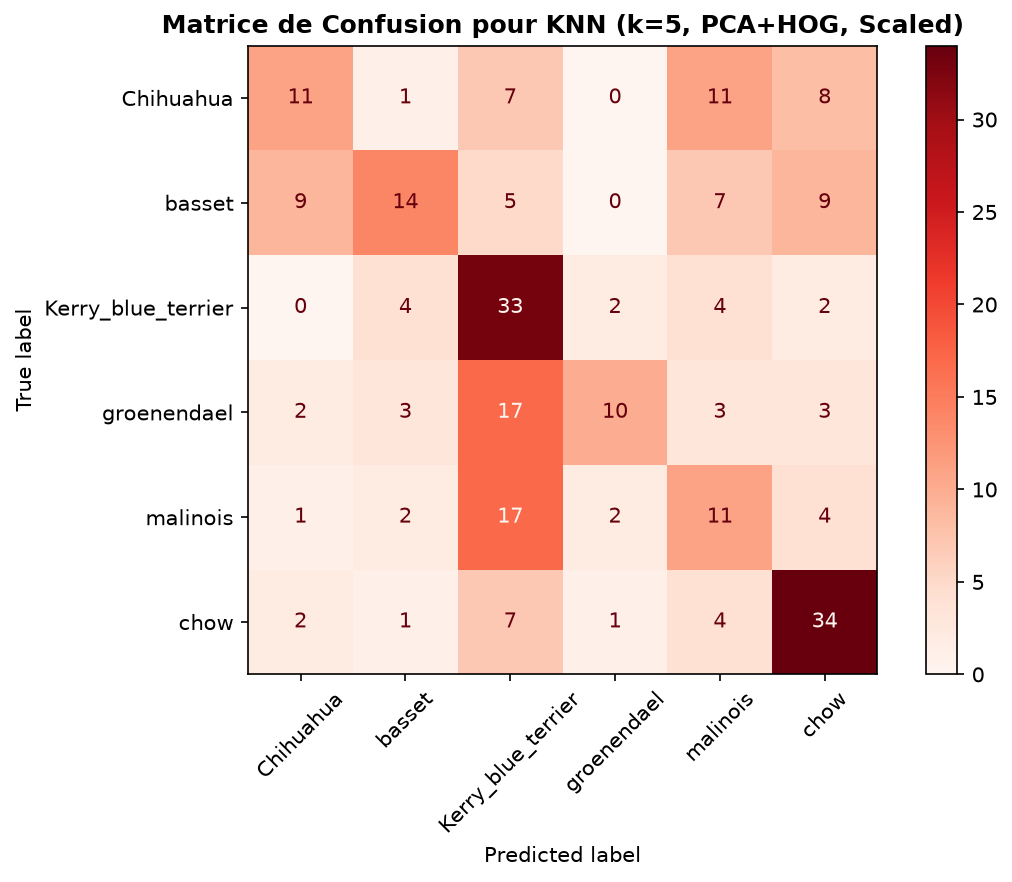
\includegraphics[width=0.55\textwidth]{confusion_matrix_knn.png}
\caption{Matrice de confusion du kNN de référence ($k=5$, PCA+HOG, normalisé). Le fait de trop prédire certaines races et pas assez d'autres vient du mélange des classes.}
\label{fig:cm_knn}
\end{figure}

\section{Classification avec le SVM}

Dans la seconde partie du projet, on a structuré notre code sous forme de pipeline Scikit-Learn (\texttt{Pipeline} et \texttt{FeatureUnion}) pour automatiser et sécuriser l'enchaînement des étapes, ce qui permet d'éviter les fuites de données (\textit{data leakage}). On remplace également le kNN par un classifieur SVM.

\paragraph{Le découpage est-il correct ?} Pour s'assurer que notre découpage train/test (\texttt{train\_test\_split} stratifié) a bien conservé la même répartition des classes, on a calculé la similarité cosinus entre les distributions empiriques de l'entraînement et du test. On obtient un score de $0{,}99995$, ce qui confirme que la proportion de chaque race est identique des deux côtés et que notre évaluation ne sera pas biaisée.

\paragraph{Réglage des paramètres.} On a cherché les meilleurs paramètres par grille de recherche (\texttt{GridSearchCV} avec validation croisée à 3 plis). Le meilleur réglage identifié est : 5 composantes PCA par classe, $C=10$ et $\gamma=0{,}005$ pour le noyau RBF.

\paragraph{Comparaison des stratégies.} Un SVM ne sait séparer que deux classes à la fois. Pour gérer six races, on compare deux stratégies : \textit{un contre un} (OvO) et \textit{un contre tous} (OvR), chacune avec un noyau linéaire puis un noyau RBF (Table~\ref{tab:svm}).

\begin{table}[H]
\centering
\caption{Pourcentage de bonnes réponses en test pour chaque stratégie SVM.}
\label{tab:svm}
\begin{tabular}{lc}
\toprule
\textbf{Stratégie} & \textbf{Bonnes réponses (test)} \\
\midrule
OvO --- noyau linéaire & $52{,}59\%$ \\
OvR --- noyau linéaire & $48{,}61\%$ \\
OvO --- noyau RBF (réglé) & $58{,}57\%$ \\
OvR --- noyau RBF (réglé) & $\mathbf{59{,}36\%}$ \\
\bottomrule
\end{tabular}
\end{table}

Le noyau RBF obtient de meilleurs résultats que le noyau linéaire, ce qui s'explique par la distribution non linéaire des classes vue précédemment (Figure~\ref{fig:scatter}). La matrice de confusion du meilleur SVM (Figure~\ref{fig:cm_svm}) montre une diagonale un peu plus marquée que celle du kNN, mais il reste de nombreuses erreurs.

\begin{figure}[H]
\centering
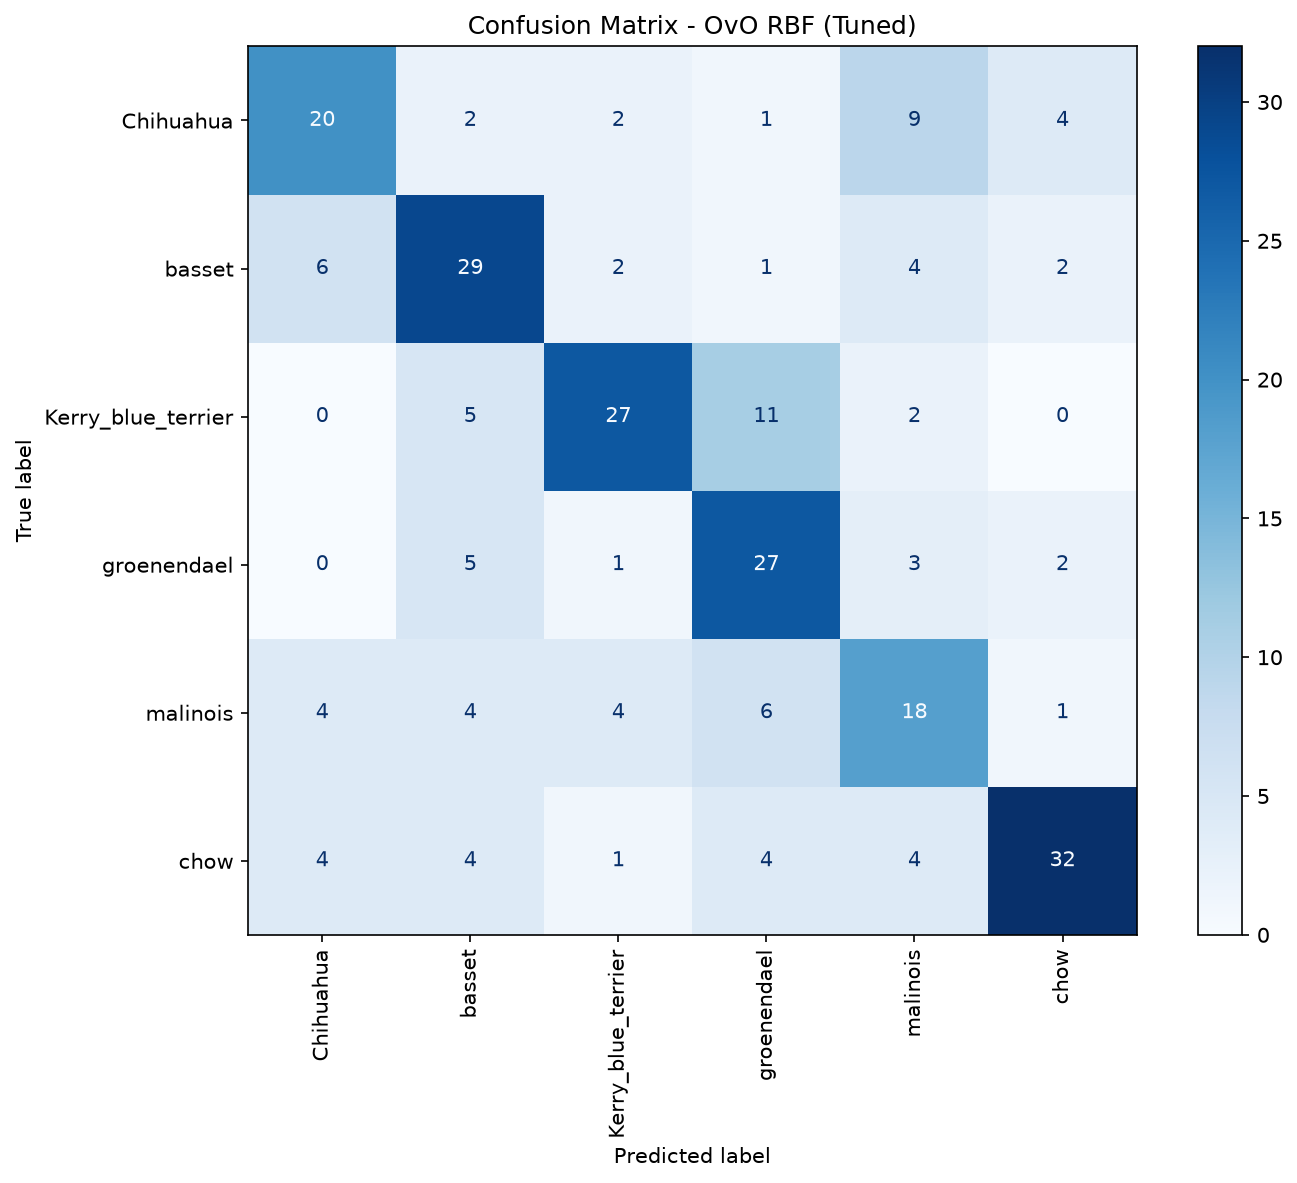
\includegraphics[width=0.62\textwidth]{confusion_matrix.png}
\caption{Matrice de confusion du SVM OvO avec noyau RBF réglé. Certaines races sont bien reconnues (forte diagonale), mais des confusions restent entre races qui se ressemblent.}
\label{fig:cm_svm}
\end{figure}

En analysant cette matrice, on remarque que la plus forte confusion a lieu entre le \textit{Kerry blue terrier} et le \textit{groenendael}. Ces deux races possèdent une morphologie proche (silhouette sombre, poils longs et touffus), ce qui rend leurs descripteurs HOG et PCA très semblables. Une solution intéressante pour y remédier serait de concevoir un classifieur binaire spécifique, entraîné uniquement à discriminer ces deux races.

\section{Discussion et piste pour aller plus loin}

\subsection{Pourquoi on plafonne sous les 60 \%}

Le kNN et le SVM plafonnent tous les deux sous la barre des $60\%$ de précision. Ce blocage ne vient pas de l'optimisation des algorithmes eux-mêmes, mais de la nature des descripteurs utilisés. La PCA et le HOG décrivent des formes globales et des contours trop génériques. Or, distinguer des races de chiens nécessite d'analyser des détails très fins (la forme des oreilles, la texture précise du pelage, la truffe). Comme nous l'avions constaté avec la projection PCA (Figure~\ref{fig:scatter}), ces descripteurs ne permettent pas de séparer les classes. Aucun classifieur classique ne peut séparer des données qui ne le sont pas au niveau de leurs descripteurs.

\subsection{Le transfer learning}

Pour dépasser cette limite, on a mis en œuvre du \textit{transfer learning} en utilisant un réseau de neurones pré-entraîné sur ImageNet (VGG16). Au lieu d'utiliser la PCA et le HOG, on utilise les couches de convolution de ce réseau comme extracteur de caractéristiques (\textit{feature extractor}).
En pratique :
\begin{itemize}
\item On gèle les poids du réseau VGG16 pour ne pas perdre l'apprentissage sur ImageNet.
\item On ajoute une couche fully-connected de classification à la fin (une couche dense de $256$ neurones suivie d'une couche softmax à $6$ sorties) que l'on entraîne sur nos images.
\item On redimensionne nos images d'origine en couleur à la taille $224 \times 224$ pixels requise par VGG16.
\end{itemize}
On a entraîné ce modèle sur 8 époques. La précision obtenue sur le jeu de test bondit à \textbf{$98\%$}, représentant seulement 5 erreurs de classification sur 251 images. La matrice de confusion obtenue (Figure~\ref{fig:cm_vgg16}) est quasiment diagonale. Ce résultat confirme que le facteur limitant du pipeline classique résidait dans les descripteurs HOG/PCA, tandis que les caractéristiques apprises par VGG16 capturent des détails discriminants bien plus riches. À noter que les six races de notre dataset font partie des classes d'ImageNet, ce qui a facilité l'apprentissage.

\begin{figure}[H]
\centering
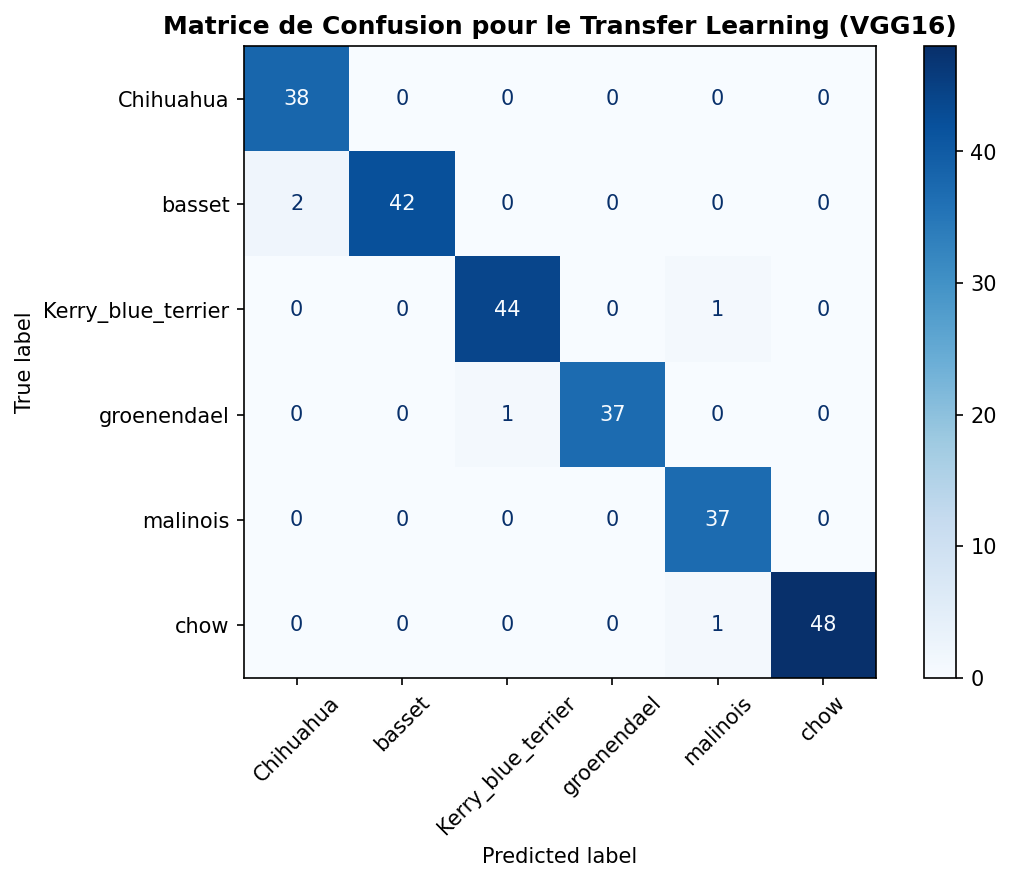
\includegraphics[width=0.7\textwidth]{confusion_matrix_vgg16.png}
\caption{Matrice de confusion du transfer learning (VGG16, couches gelées). La diagonale est presque parfaite : $98\%$ de bonnes réponses, contre $\sim59\%$ pour les méthodes classiques.}
\label{fig:cm_vgg16}
\end{figure}

\section{Conclusion}

En conclusion, on a mis en place une chaîne complète de traitement d'images, allant du rognage des photos selon leurs boîtes englobantes jusqu'à l'évaluation de classifieurs kNN et SVM. Ce projet nous a permis de mettre en pratique plusieurs notions clés du cours de Machine Learning : l'importance du centrage-réduction des descripteurs, la gestion du compromis biais-variance, et la stratification lors du découpage train/test. On a pu constater que la qualité de l'extraction des caractéristiques détermine la performance maximale du classifieur. Les descripteurs classiques (PCA, HOG) se révèlent trop limités face à des classes morphologiquement proches, plafonnant à environ $59\%$ de précision. L'utilisation du transfer learning avec VGG16 a permis d'illustrer la puissance des descripteurs appris par apprentissage profond, portant notre taux de réussite à $98\%$.

\end{document}
